\section{Theoretischer Hintergrund}

Internet of Things (IoT) ist ein Gebiet, welches dem Alltag viele Vorteile bringt. Durch die Möglichkeit
Geräte aus dem Alltag mit dem Internet zu verbinden, birgt IoT aber auch Sicherheitslücken die besagte Geräte sehr Gefährlich
werden lässt. Um dem entgegen zu wirken soll sich die Dissertation im Gebiet der Malwareforschung befinden. Im speziellen soll es dabei um 
die Erkennung von Botnetzen gehen, welche Angriffe über IoT-Geräte ausführen. \\
Ein Botnetz ist der Zusammenschluss von Hosts, auch Bots oder Zombies genannt, gesteuert von einem Angreifer, auch Botmaster genannt in einem 
Overlay-Netzwerk \cite{Xing2021SurveyOB}. Die Botnetze nutzen Zero-day Schwachstellen, Peer-2-Peer Netze, Phishing Angriffe, Anonyme Netzwerke,
Blockchain Netzwerke und Stromnetze zur Verbreitung und ihrer Verwendungszwecke \cite{DBLP:conf/cycon/CasenoveM14,DBLP:conf/esorics/KurtECAU20}. Auf Basis der Architektur 
des Botnetzes findet zu jeder Zeit ein Kommunikations- und Kontrollprozess mit dem Command und Control (C\&C)-Server statt. Der C\&C-Server gibt den Bots Befehle die 
diese dann durchführen \cite{SCHILLER200729} zum Beispiel, über das Internet Relay Chat (IRC)-Protokoll. \\ Botnetze durchlaufen drei Phasen wie Wazzan et al. 
\cite{Wazzan2021InternetOT} beschreiben, scannen, ausbreiten und angreifen. Während der Scan-Phase sucht ein Bot nach vulnerablen IoT-Geräten und 
infiziert das Gerät entweder durch brute force Methoden oder durch Ausnutzen einer Schwachstelle.
In der Ausbreitungs-Phase ist eine lauffähige Version des Bots installiert und auf Basis der Architektur des infizierten Geräts ausgeführt.
Um auf dem Gerät Malware zu verhindern die nicht vom Botnetz selbst ausgeführt wird, stoppt der Bot andere Prozesse um Ports für sich selbst zu blocken. 
Daraufhin rekrutiert das bösartige Programm weitere Bots um das Botnetz so schnell wie möglich zu erweitern. In der Angriffs-Phase führt das Botnetz Angriffe wie Distributed Denial of 
Service (DDoS), crypto mining und spam Angriffe aus. Die erläuterten Phasen beschreiben auch Studien wie 
\cite{10.1007/978-3-030-33229-7_21, Alzahrani2020,DBLP:journals/computer/VlajicZ18,NGUYEN2020128}. \\
Nach der Erläuterung wie Botnetze funktionieren wäre nun zu fragen, wie der Prozess eines Botnetzes erkennbar ist um IoT-Geräte entsprechend zu schützen. 
Nach Xing et al. \cite{Xing2021SurveyOB} kann die Botnetz Erkennung in Honeypot Analyse, Signaturen aus der Kommunikation und abnormales Verhalten klassifiziert
werden. Wie Abbildung \ref{fig:bot_det_met} zeigt, unterteilen diese Klassifikationen Methoden zur Erkennung. 

\begin{figure}[b!]
    \centering
    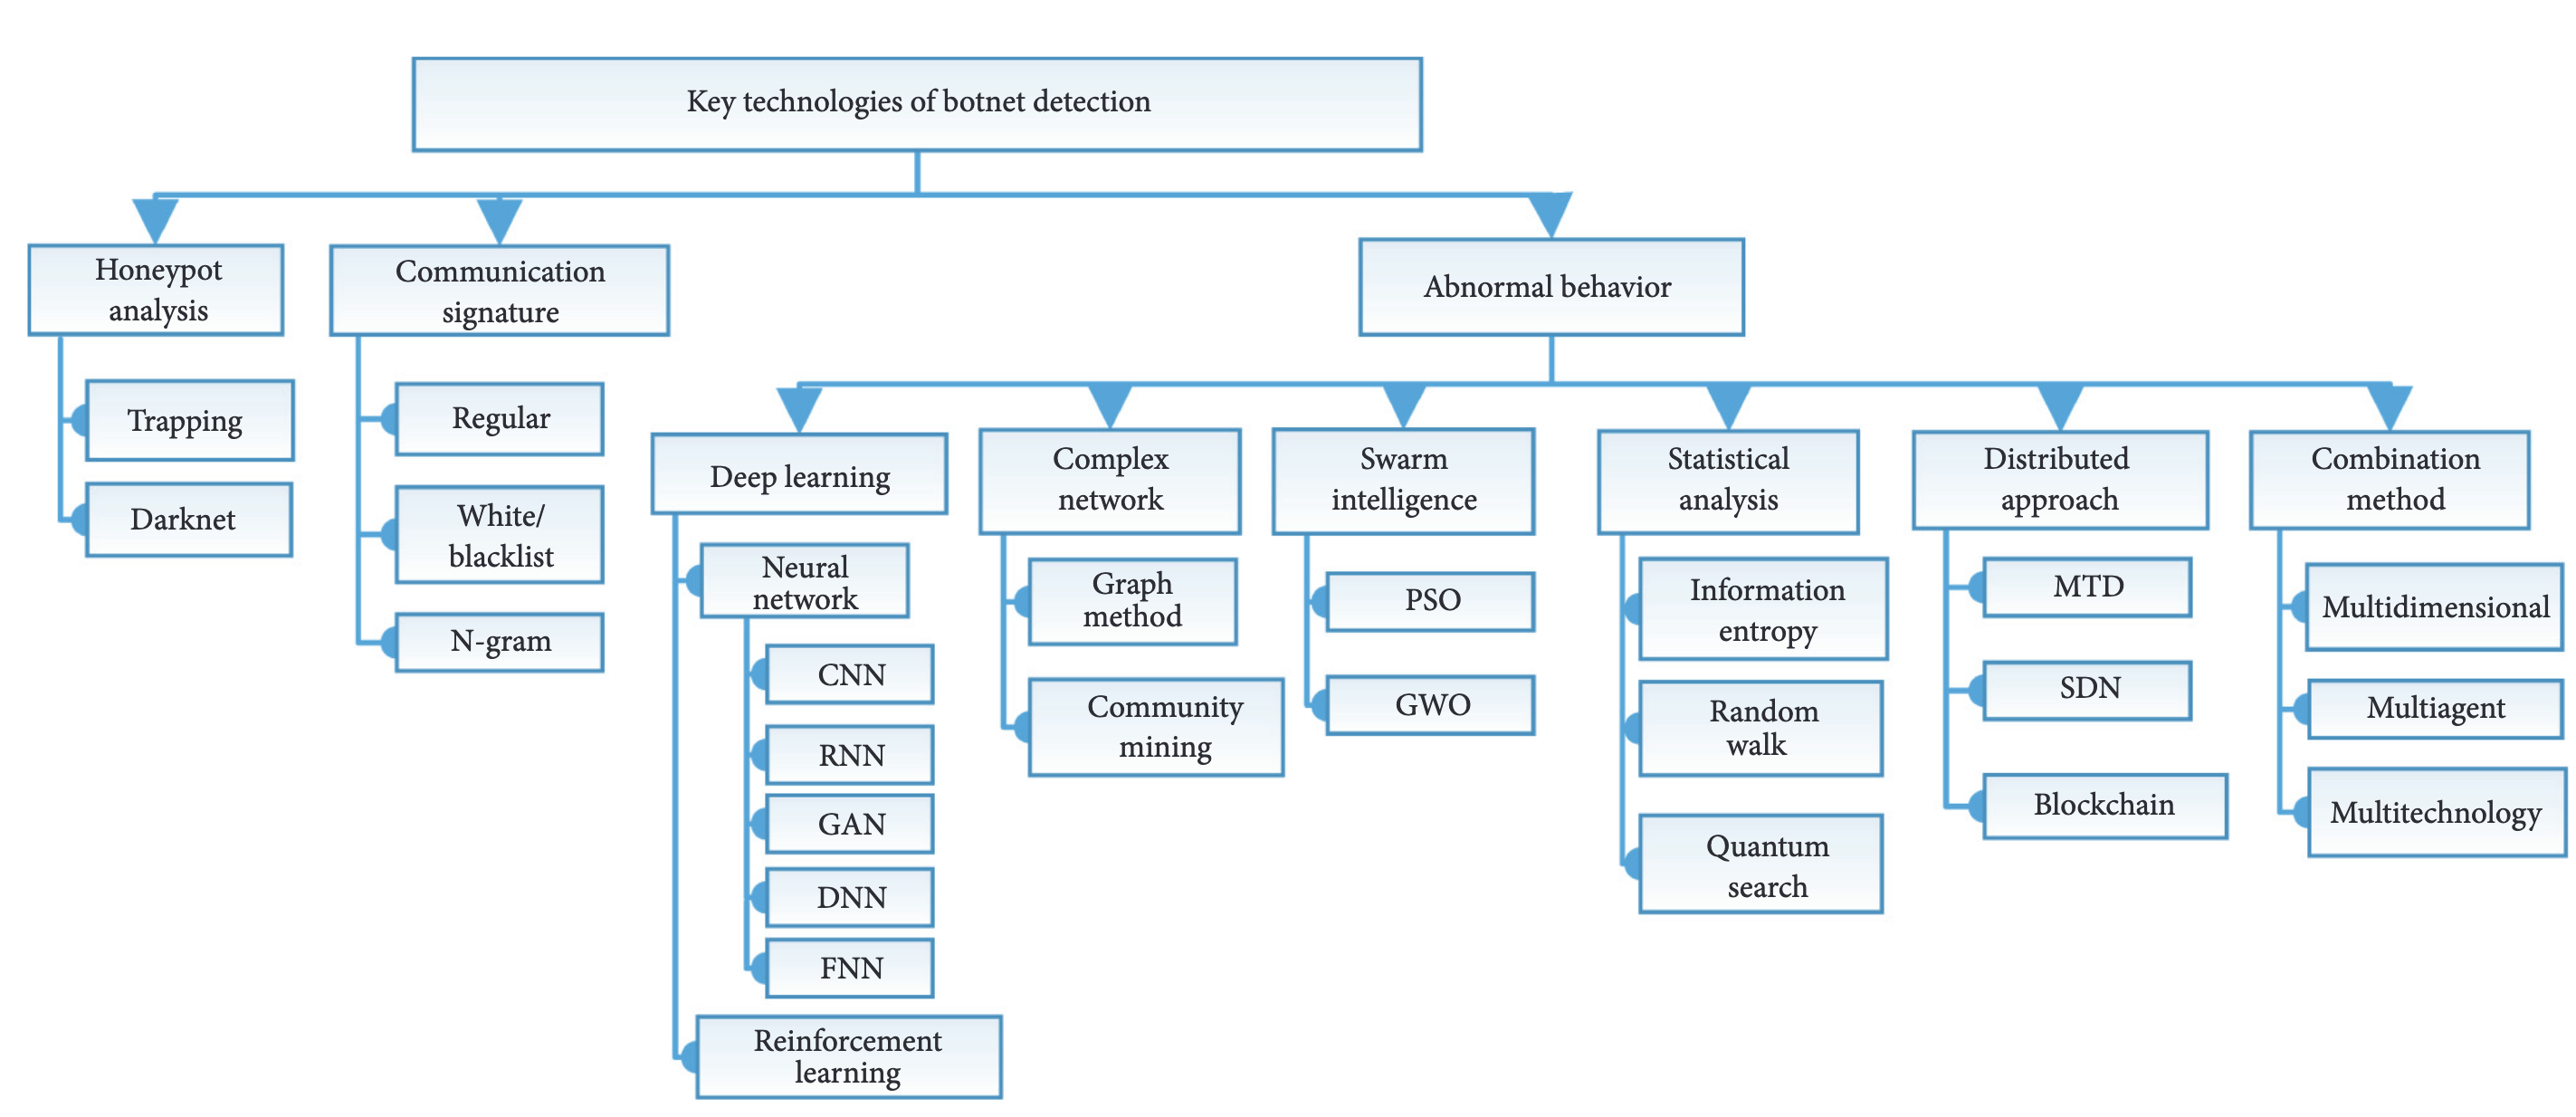
\includegraphics[scale=0.314]{./pictures/botnet_detection_methods.png}
    \caption{Klassifizierte Erkennungsmethoden von Botnetzen (übernommen von \cite{Xing2021SurveyOB}).}
    \label{fig:bot_det_met}
\end{figure}

Die \textit{Honeypot Analyse} erkennt Code Beispiele durch das Honeypot trapping was eine hohe Genauigkeit von bereits bekannten Botnetzen ermöglicht. Die Honeypot Methoden können
verschlüsselten Netzwerkverkehr nur schlecht erkennen sowie unbekannte Botnetze. Bots die eigene Funktion zur Umgehung von Honeypots besitzen, können durch fehlende Benutzereingriffe
auch nicht von der \textit{Honeypot Analyse} erfasst werden. Weit verbreitet sind die Methoden Erkennung von \textit{Kommunikationssignaturen} anhand von Signaturen und Muster. Dabei 
werden in Intrusion Detection Systems (IDS) Regeln für den Merkmalsabgleich hinterlegt um Botnetz aktivitäten zu identifizieren. Dadurch können IDS Botnetze mit bestimmten Merkmalen 
erkennen, aber unbekannte Funktionen werden dabei nicht erkannt sowie auch Botnetze die Techniken zur Verschleierung von Code nutzen. Bei den Methoden die durch 
\textit{abnormales Verhalten} ist die Idee, Hostverhalten oder Netzwerkverkehr Auffälligkeiten zwischen gutartigem und bösartigem Verhalten zu erkennen. Neben den erwähnten Methoden 
erläutern Singh et al. \cite{DBLP:journals/compsec/SinghSK19} Techniken, zur Erkennung von Botnetzen. Singh et al. klassifizieren die Techniken in Flow-, Anomalie-, Flux-, DGA-basierten und
Bot infizierungs Erkennung. Die Umsetzung mit mehreren Erkennungsstufen erklären Stevanovic und Pedersen \cite{DBLP:journals/ijcysa/StevanovicP16}. Diese Erkennung soll mehr Geräte vor der illegalen Verwendung schützen.

% - Welche Erkennungen gibt es zu welcher Phase?

% - Vielleicht ein ML Modell implementieren was via SDN ein IoT Netzwerk überwacht
% - Das ganze z.B. mit Mirai testen in einem Labor
% - Laborexperiment
% - ML Modell -> Vielleicht Unsupervised Learning, passenden Algorithmus raussuchen (basierend auf den besten Erkennungsmethoden durch ML)
% - Das Paper im Auge behalten für entsprechende Begriffe
% - WAS IST DAS ZIEL? - Welche Ergebnisse will ich am Ende haben?
% - Ist ein Zusammenhang wichtig, wofür das Botnet verwendet werden soll?
% - Ich will die Erkennung von Botnetzen verbessen (Ergebnisse sollen darauf beruhen) - Wurde die Erkennung durch meine Diss verbessert?
% - Mehrere Level der Erkennung während jeder Botnetzphase
% - Im aktuellen Stand der Forschung auf die Hauptgebiete aus der Einführung eingehen
% - Level: Host-, Network-, (DNS, Anomaly) based-approach -> auf Basis einer der Techniken, mehrere Protokolle etc. beobachten

